% ==============================================
% CFD Tutorial Template: OpenFOAM Terminal Basics
% Class: scrartcl (KOMA-Script) - optimized for tutorials
% Content: orificePlate with simpleFoam
% ==============================================

\documentclass[
    parskip=half,      % Space between paragraphs (better for steps)
    DIV=12,            % Optimal margins for readability
    headings=normal,   % Professional heading sizes
    fontsize=11pt,     % Slightly larger for screen reading
    english            % Language setting
]{scrartcl}

% ========== ESSENTIAL PACKAGES ==========
\usepackage[utf8]{inputenc}
\usepackage[T1]{fontenc}
\usepackage{lmodern}
\usepackage{geometry}
\usepackage{tikz}
\usepackage{microtype}           % Superior typography
\usepackage{graphicx}            % For screenshots (optional)
\usepackage{xcolor}              % Color coding
\usepackage{listings}            % Code listings
\usepackage{siunitx}             % Proper units: \si{\meter\per\second}
\usepackage{amsmath}             % Math equations
\usepackage{hyperref}            % Clickable links
\usepackage{url}
\usepackage{booktabs}            % Professional tables
\usepackage{caption}             % Better figure captions
\usepackage[english]{babel}
\usepackage{float}

% ========== CUSTOM COLORS ==========
\definecolor{codebg}{RGB}{240, 245, 250}
\definecolor{cmdcolor}{RGB}{0, 100, 0}
\definecolor{outputcolor}{RGB}{100, 100, 150}
\definecolor{warningcolor}{RGB}{180, 0, 0}
\definecolor{tipcolor}{RGB}{0, 100, 50}

% ========== CODE LISTING SETUP ==========
\lstset{
	backgroundcolor=\color{codebg},
	basicstyle=\ttfamily\small,
	breaklines=true,
	frame=single,
	captionpos=b,
	rulecolor=\color{gray!30},
	tabsize=2,
	showstringspaces=false
}

% Custom style for terminal commands
\lstdefinestyle{terminal}{
	basicstyle=\ttfamily\small\color{cmdcolor},
	backgroundcolor=\color{black!5},
	frame=none,
	columns=fullflexible
}

% Custom style for OpenFOAM files
\lstdefinestyle{openfoam}{
	language=C++,
	morekeywords={dimensions, internalField, boundaryField, type, value},
	keywordstyle=\color{blue},
	commentstyle=\color{gray!50}\itshape
}

\lstdefinestyle{output}{
	backgroundcolor=\color{black!5},
	basicstyle=\ttfamily\small\color{outputcolor},
	frame=none,
	breaklines=true
}
% ========== HYPERREF SETUP ==========
\hypersetup{
	colorlinks=true,
	linkcolor=blue,
	citecolor=green,
	filecolor=magenta,
	urlcolor=cyan,
	pdftitle={OpenFOAM Tutorial: pitzDaily with simpleFoam},
	pdfauthor={Your Name},
	pdfsubject={CFD with OpenFOAM},
	pdfkeywords={OpenFOAM, CFD, simpleFoam, pitzDaily, terminal}
}


\newcommand{\warning}[1]{\par\vspace{5pt}\noindent\textcolor{red}{\textbf{WARNING:}} #1\par\vspace{3pt}}
\newcommand{\tip}[1]{\par\vspace{5pt}\noindent\textcolor{green!50!black}{\textbf{TIP:}} #1\par\vspace{3pt}}
\newcommand{\important}[1]{\par\vspace{5pt}\noindent\textcolor{blue}{\textbf{IMPORTANT:}} #1\par\vspace{3pt}}                    

% ========== CUSTOM COMMANDS ==========
\newcommand{\terminalcmd}[1]{\textbf{\texttt{\textcolor{cmdcolor}{#1}}}}
\newcommand{\ofkeyword}[1]{\textbf{\textcolor{blue}{#1}}}
\newcommand{\filename}[1]{\texttt{\textcolor{purple}{#1}}}
\newcommand{\commandexample}[1]{\vspace{5pt}\hspace{10pt}\terminalicon\ \terminalcmd{#1}\vspace{5pt}}
\newcommand{\key}[1]{\texttt{\textbf{#1}}}

\usetikzlibrary{patterns}
% ========== DOCUMENT START ==========
\begin{document}

% ========== TITLE PAGE ==========
\title{Tutorial \#3: Orifice plate}
\subtitle{Axisymmetrical Flow: Orifice Plate with simpleFoam}
\subject{Open Source CFD }
\author{Robert Castilla \\ Department of Fluid Mechanics}
\date{2025-26 \\ Version 1.0}
\publishers{Learning Objectives:
\begin{itemize}
    \item Create a blockMesh dictionary with python
    \item Extrude the mesh to create a axisymmetrical simmulation
    \item Run a simple steady-state simulation
    \item Monitor residuals from terminal
    \item Analyze basic results in terminal and paraview
    \item Validate results with standard publication
\end{itemize}}

\maketitle

% ========== ABSTRACT ==========
\begin{abstract}
This tutorial introduces the use of a python interface to create a blockMesh dictionary. 
The study case is the a simple orifice plate, which will be simulated with \terminalcmd{simpleFoam}. It is not available in tutorials and it will 
be generated from a template case. Pressure loss and dimensionless coefficient will be obtained
both with post-processing utilities in terminal and with paraview.
\end{abstract}

\tableofcontents
\newpage

% ========== SECTION 1: INTRODUCTION ==========
\section{Introduction and Theoretical Background}

\subsection{What is an orifice plate?}
An orifice plate is a device used to experimentally measure the flow rate in a pipe. 
It is basically a circular plate, with an orifice in the center, that restricts the
flow and produce a pressure loss. This pressure loss is mathematically related to the
flow rate in the pipe.


\begin{figure}[h]
	\begin{center}
		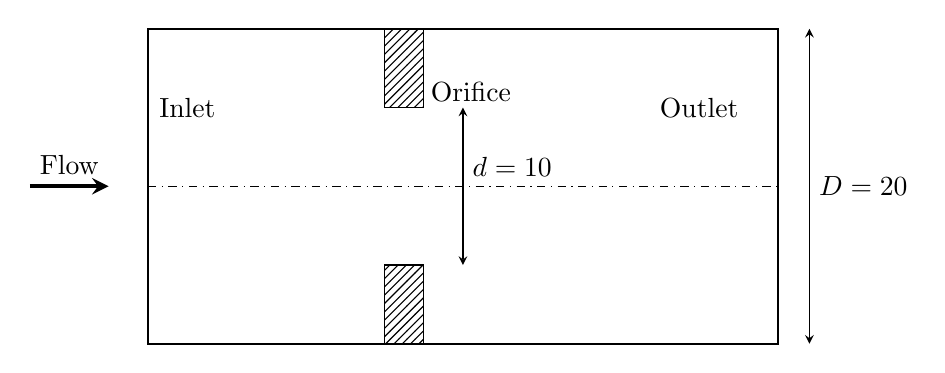
\begin{tikzpicture}[scale=1,> = stealth]
			% Simple orifice plate
			\draw[thick] (0,-2) rectangle (8,2);
			\draw[dash dot] (0,0) -- (8,0);

			
			% Plate
			\draw[pattern=north east lines] (3,1) rectangle (3.5,2);
			\draw[pattern=north east lines] (3,-1) rectangle (3.5,-2);
			
			
			% Flow arrow
			\draw[-stealth, ultra thick] (-1.5,0) -- (-0.5,0) node[midway,above] {Flow};
			
			% Labels
			\node at (0.5,1) {Inlet};
			\node at (7,1) {Outlet};
			\node at (4.1,1.2) {Orifice};
			
			% Dimensions
			\draw[<->] (8.4,-2) -- node[right] {$D = 20$} (8.4,2);
			\draw[<->] (4,1) -- node[above right] {$d = 10$} (4,-1);
		\end{tikzpicture}
	\end{center}
	\caption{Orifice plate geometry. Dimensions are in mm.}
\end{figure}

More information can be found on  \hyperlink{https://en.wikipedia.org/wiki/Orifice_plate}{Wikipedia}.
\subsection{Flow rate measurement}

In the orifice plate flow rate is computed with equation \eqref{eq:FR}

\begin{equation}
	\label{eq:FR}
	Q = C_d \frac{A_o}{\sqrt{1-\beta^4}}\sqrt{\frac{2\Delta p}{\rho}}
\end{equation}

where $\beta = d/D$,$A_o$ is the area of the orifice, $\rho$ is the density of the fluid
, $\Delta p$ is the pressure loss in the orifice and $C_d$ is the \textbf{coefficient
of discharge}. The approximate value of $Cd$ is 0.6, but it can be more precisely
estimated with the Reader-Harris/Gallagher equation

\begin{equation}
	\begin{split}
		C_d = & 0.5961 + 0.0261\beta^2 - 0.216\beta^8 + 0.000521\left(\frac{10^6\beta}{Re_D}\right)^{0.7} \\
		& + (0.0188 + 0.0063A)\beta^{3.5}\left(\frac{10^6}{Re_D}\right)^{0.3} \\
		& + (0.043 + 0.080e^{-10L_1} - 0.123e^{-7L_1})(1 - 0.11A)\frac{\beta^4}{1-\beta^4} \\
		& - 0.031(M'_2 - 0.8{M'_2}^{1.1})\beta^{1.3} + 0.011(0.75 - \beta)\left(2.8 - \frac{D}{0.0254}\right)
	\end{split}
\end{equation}
where
\begin{align*}
	\beta &= d/D \quad \text{(diameter ratio)}\\
	Re_D &= \text{Reynolds number based on pipe diameter}\\
	A &= \left(\frac{19000\beta}{Re_D}\right)^{0.8}\\
	M'_2 &= \frac{2L'_2}{1-\beta}
\end{align*}

The value of $\Delta p$ depends on where the pressure are measured upstream and downstream
with relation to the orifice. In this case we are going to measure the pressure upstream
($p_1$) at a distance $D$ and downstream ($p_2$) at a distance $\frac{D}{2}$.
According to ISO 5167 standard, for this case $L'_1 = 1$ and $L'_2 = 0.47$. 


\section{Simulation of the flow in the orifice plate}
\subsection{Case Overview}

\begin{table}[H]
	\centering
	\begin{tabular}{@{}ll@{}}
		\toprule
		\textbf{Parameter} & \textbf{Value} \\
		\midrule
		Solver & \terminalcmd{simpleFoam} (steady, incompressible) \\
		Turbulence model & $k$-$\omega$ - SST  \\
		Flow regime & Turbulent \\
		Geometry & orifice plate \\
		Reynolds number & $ 2 \times 10^4$ (based on pipe diameter) \\
		Expected runtime & 60-80 seconds \\
		\bottomrule
	\end{tabular}
	\caption{Orifice plate case specifications}
	\label{tab:case_specs}
\end{table}

\subsection{Case copy}

Since this case is not available in the tutorials folder, we have two options. We can
either adapt a tutorial (for instance, the pitzDaily tutorial) or we can use a 
\texttt{template} case, that can be found in \filename{\$FOAM\_ETC/templates}. 

\begin{lstlisting}[style=terminal]
	# load OpenFOAM if it is not included in the .bashrc file
	source /usr/lib/openfoam/openfoam-2312/etc/bashrc
	
	# Make a local folder
	mkdir -p ~/Tutorials/Tutorial_3
	
	# Copy the inflowOutflow in this folder
	cp -r $FOAM_ETC/inflowOutflow ~/Tutorials/Tutorial_3/orificePlate
	# Note that we have changed the name with the copy
	
	# Go to the tutorial place
	cd ~/Tutorials/Tutorial_3/orificePlate
\end{lstlisting}

This case is a simple example of a fluid domain with an inlet and an outlet. In the
\filename{README} file you can read the instructions to use the template. It is intended
to be used with a general 3D geometry meshed with \terminalcmd{snappyHexMesh}. Since
we are going to use \terminalcmd{blockMesh} with an axisymmetrical mesh, this file 
can be removed

\begin{lstlisting}[style=terminal]
	# remove the README file
	rm README
\end{lstlisting}

\vspace{1cm}
\noindent
\textbf{Acknowledgments:} The author acknowledges the assistance of 
\href{https://deepseek.com/en}{DeepSeek}, an AI assistant created by DeepSeek Company, 
for providing valuable support in structuring this document, formatting LaTeX code, 
and developing the tutorial content.

\textbf{Disclaimer:} All content has been reviewed, modified, and 
validated by the author. The author takes full responsibility for 
the accuracy, completeness, and educational quality of this material. 


% ========== END DOCUMENT ==========
\end{document}